\documentclass[12pt, oneside]{extbook} % the document type needs to be change
\usepackage{geometry}
\usepackage{listings}
\usepackage{graphicx}
\usepackage[utf8]{inputenc}
\usepackage[T1]{fontenc}
\usepackage[italian]{babel}

\geometry{
    top = 1.5cm,
    bottom = 1.5cm,
    left = 2cm,
    right=2cm,
}

\begin{document}

\chapter*{BGP Security}

\section{Introduzione - possibili vulnerabilità}
La sicurezza di BGP è ancora un argomento molto importante, in particolare con BGP hijacking etc...
\\Ci sono due famiglie di vulnerabilità:
\begin{itemize}
    \item BGP gira su TCP, quindi ci sono i problemi di sicurezza legati a TCP/IP;
    \item il secondo tipo di problema dipendono dal fatto che dobbiamo certificare un prefisso e l'AS che c'è dietro
\end{itemize}

\section{Vulnerabilità legate a IP/TCP}

\subsection{Peer spoofing and TCP reset}
Siccome BGP gira su TCP/IP c'è un problema di autenticazione, quindi i messaggi BGP possono essere spoofati come se fossero mandati da un peer reale, questa è però una vulnerabilità teorica: il provider forza dei meccanismi di anti-spoofing per evitare che ad esempio da casa mando un messaggio BGP spoofato.
\\C'è un caso speciale di messaggi di spoofing che è il reset attack: se la connessione TCP non è sicura, si può pensare di resettare la connessione TCP e fare un reset della connessione TCP tramite un messaggio BGP è un grosso DoS, se un peer perde la connessione con un altro peer tutte le rotte che vengono considerate down sono ritirate e l'informazione viene propagata agli altri peers e ci vogliono minuti per rimettere tutto a posto.
\\Per risolvere i problemi, per resettare una connessione serve conoscere il seq number del messaggio TCP, quindi non è così semplice ma in ogni caso la prima contromisura a questi attacchi è la strong sequence number randomization.
\\Quindi, la seconda vulnerabilità prevede che basti semplicemente spoofare l'IP address, inoltre una connessione TCP può essere resettata anche con ICMP e qui non era neanche necessario conoscere il seq number, ma di nuovo ci sono varie contro-misure.

\subsection{Session hijack}
Per l'hijack della sessione, siamo ancora in un caso di peer spooofing, ma in realtà l'idea è di entrare in una sessione già stabilita, quindi è ancora più complicato.
\\Ci sono le stesse contro-misure di prima, 10 anni fa è stato suggerito di usare IPsec ma oggi non si usa.
\subsection{Contromisure}
\subsubsection{MD5 signature}
L'md5 signature option è un opzione TCP che può essere usata per proteggere delle sessioni TCP, quindi si aggiunge un MAC ai pacchetti TCP, usando una chiave simmetrica (è un HMAC).
\\C'è la nuova versione di questa opzione che è la TCP Authentication Option, dove la funzione di hash è negoziabile, inoltre vengono fornite altre cose come una migliore generazione delle chiavi, derivate da una singola chiave mater, inoltre si può cambiare la chiave in una stessa sessione.
\\Non si può quindi spoofare una sessione TCP perché non si ha la chiave, è solo autenticazione ma il problema è che lo standard non ha specificato come negoziare la chiave.
\\Abbiamo quindi un problema di autenticazione, non c'è IPsec/TLS, non serve l'entryption e si può risolvere autenticando la connessione TCP con questa opzione, sia quella vecchia che quella nuova.

\subsubsection{TTL hack}
TTL hack è un'altra contromisura, l'idea è che un peer esterno BGP è ad un hop di distanza, su un p2p link dedicato oppure in una rete interna.
\\Per iBGP è diverso ma in generale il numero di hop è limitato quindi se si conosce questo numero di hop si può controllare il valore del TTL quando si riceve un messaggio BGP: i peer fanno agreement su un certo valore di TTL, se si scende sotto una certa threshold il messaggio BGP viene buttato.
\\L'idea è che per peer vicini sono gestiti dagli operatori, peer più lontani possono essere quelli da dove parte l'attacco infatti il problema non è della home network perché tutti gli operatori usano meccanismi anti-spoofing quasi sempre, ma da altri AS ci può essere il problema, ma ci sono molti hop da altri AS.

\subsection{Vulnerabilità: route flapping}
Cambio ripetitivo alla routing table BGP, una route flap occorre quando una rotta viene rimossa e poi re-advertised e se avviene ad un tasso elevato può portare diversi problemi ai router perché tutte le withdraw vengono propagate a tutti gli altri peers.
\\Se avviene abbastanza velocemente, quindi ad esempio 30-50 volte per secondo il router è sovraccarico, il danno potenziale è lo slow down o anche drop dei pacchetti.
\\La contromisura è il route damping, quindi c'è una finestra temporale per cui si usa un algoritmo che genera un backoff esponenziale per cui si ignora la rotta inviata.
\\Viene quindi aggiunto questo valore di penalità ogni volta che avviene un evento di flapping, posta dai peer ed aggiunta ad un totale per il flapping router.
\\Tale penalità decade esponenzialmente nel tempo (è appunto un backoff), ma se il flap persiste abbastanza nel tempo, il totale eccede una certa thrsehold configurabile.
\\Se invece non vengono più osservati flap, la penalità raggiunge una threshold di riuso.
\\Da un certo punto di vista mitiga il problema ma da un punto di vista di attaccante può incrementare il DoS.

\subsection{IPSec per BGP}
IPsec per BGP? Qualcuno ha suggerito di usarlo, ma la realtà è che BGP ed IPsec non vanno d'accordo in reti reali, per diverse ragioni.
\\Abbiamo comunque avuto problemi di BGP hijacking dovuti a configurazioni sbagliate dovute ad errori umani, ma anche per vulnerabilità software, servono quindi protezioni che certifichino cosa c'è scritto nel messaggio BGP: crypto binding fra l'AS ed il prefisso BGP


\section{Vulnerabilità del control plane BGP}
\subsection{Prefix hijacking}
Si fa hijack del prefisso, quindi l'attaccante comincia a fare annunci per un AS che in realtà lui non è.
\\Ci sono due conseguenze:
\begin{itemize}
    \item si può fare un MiTM
    \item si può anche fare un DoS
\end{itemize}
Immagine rappresentativa:\\
\begin{figure}[h!]
    \centering
    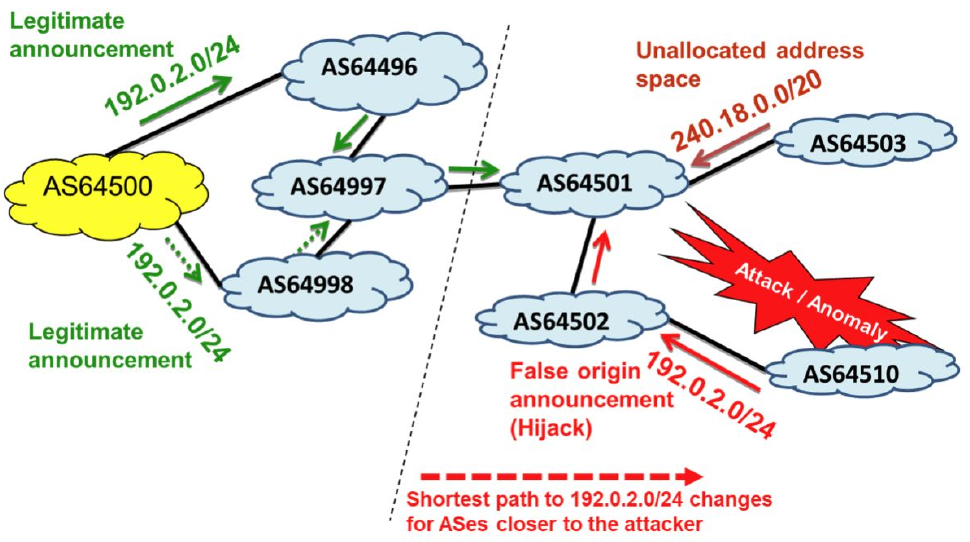
\includegraphics[scale=0.5]{../../immagini/perf_hijack}
\end{figure}\\\\
Può avvenire quando un AS accidentalmente o malevolmente genera ed annuncia un prefisso che non è il suo.
\\Alcuni AS quindi vedranno dei path più corti e preferiranno la rotta annunciata dall'AS che fa hijack, che quindi ruberà i pacchetti destinati all'altro.
\\È possibile farlo funzionare per tutti gli AS, non serve nemmeno rubare tutto il prefisso, se questo è più lungo tutti i router installeranno quella rotta perché il prefisso sarà più lungo, quindi quando si fa hijacking si annuncia una rotta con prefisso più lungo.
\\Le conseguenze dell'attacco sono
\begin{itemize}
    \item DoS: il pacchetto viene droppato dall'attaccante
    \item eavesdropping: l'attaccante può vedere i pacchetti
    \item misdirection verso server impostori, stiamo comunque facendo impersonificazione o MiTM, possiamo far credere di essere dei server legittimi
\end{itemize}

Ci sono vari problemi ogni anno:
\begin{itemize}
    \item Dicembre 2017: un AS russo ha fatto hijacking di 80 prefissi ad alto traffico di Google, Facebook, Riot Games e Twitch TV;
    \item ...
\end{itemize}
\subsubsection{Contromisure}
La prima contromisura per questo tipo di attacco è il BGP filtering, se tutti gli AS implementassero filtering fare hijacking sarebbe impossibile: bisogna fare filtering su messaggi in ingresso ma anche in uscita perché possono esserci errori; si filtrano prefissi che vengono da AS reali.

\subsection{BGP UPDATE modification}
Modifichiamo un UPDATE ricevuto da una altro peer e si può modificare qualunque cosa, come l'AS path inserendo il proprio AS oppure cambiando path e siccome non c'è autenticazione nessuno può effettuare controlli.
\\Quello che quindi può fare un AS malevolo è rimuovere da un BGP update riceuto alcuni degli AS precedenti nell'AS\_PATH per far si che questo sembi più corto.
\\Un avversario modifica il prefisso sempre con lo stesso obiettivo, ovvero quello di fare hijacking delle rotte, magari per cercare di incrementare i guadagni dai clienti o per fare eavsedropping del traffico
\\Un altro modo prevede di rimpiazzare il prefisso dell'update ricevuto con uno più specifico e poi forwardare ai vicini.
\\L'attacco è di Kapela-Pilosov: viene cambiato solo il prefisso, quindi il path rimane inalterato.
\\Questo implica che gli AS nell'Internet accetteranno l'update ed useranno l'AS avversario, fatta eccezione per gli AS che sono nel path che va dall'avversario al prefisso, in quanto ci sarà la detection dei loop standard di BGP.

\subsection{Route leaks}
Un leak non è per forza un attacco: il significato è che si fa advertising di un prefisso per cui non si dovrebbe.
\\Tipicamente, non tutte le rotte sono richieste dai peers, dipende dalla natura del collegamento fra peers: se c'è un customer di un AS, non è detto che debba conoscere tutte le rotte verso gli altri.
\\Quindi un root leak prevede che un AS rubi un update, tipicamente ad esempio un customer non direbbe mai le sue rotte.
\\La local preference è un attributo che ha una priorità maggiore valore fra gli attributi, quindi quando un customer manda un messaggio BGP tipicamente ha la local preference più alta e quindi verrebbe scelto nella rotta per prendere tutto il traffico\\
\begin{figure}[h!]
    \centering
    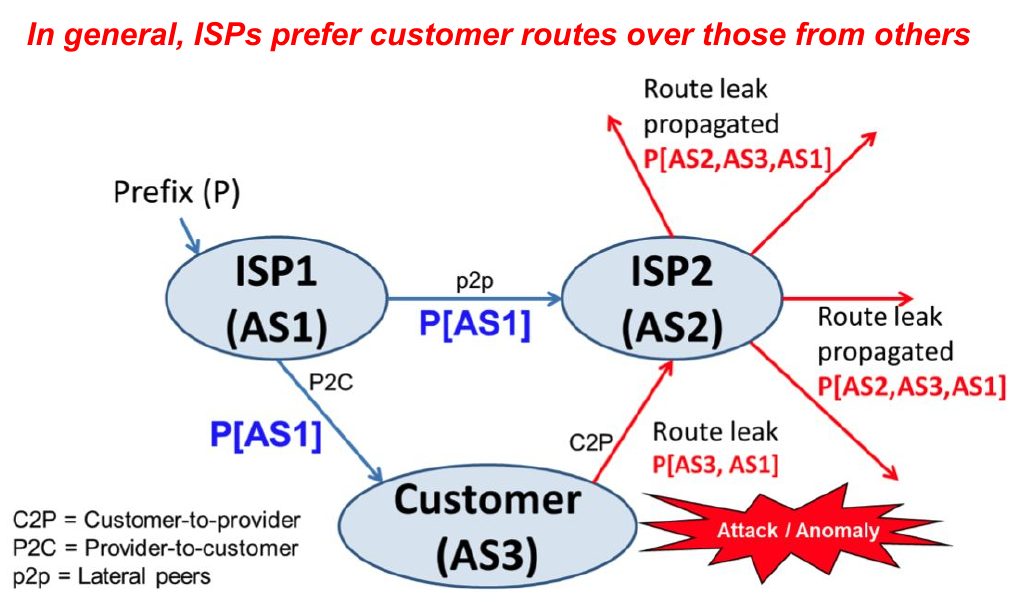
\includegraphics[scale=0.5]{../../immagini/route_leaks}
\end{figure}
questo leak quindi rompe quelli sono gli agreement fra i peers.
\\È simile all'hijacking, ma gli obiettivi sono diversi.
\\In ogni caso, entrambi i problemi hanno come soluzione il filtering in modo da non accettare tutti gli announcements che vengono filtrati.

\section{Tipologie di BGP peers e relazioni fra essi}
Ci mettiamo dal punto di vista dell'AS arancione:\\
\begin{figure}[h!]
    \centering
    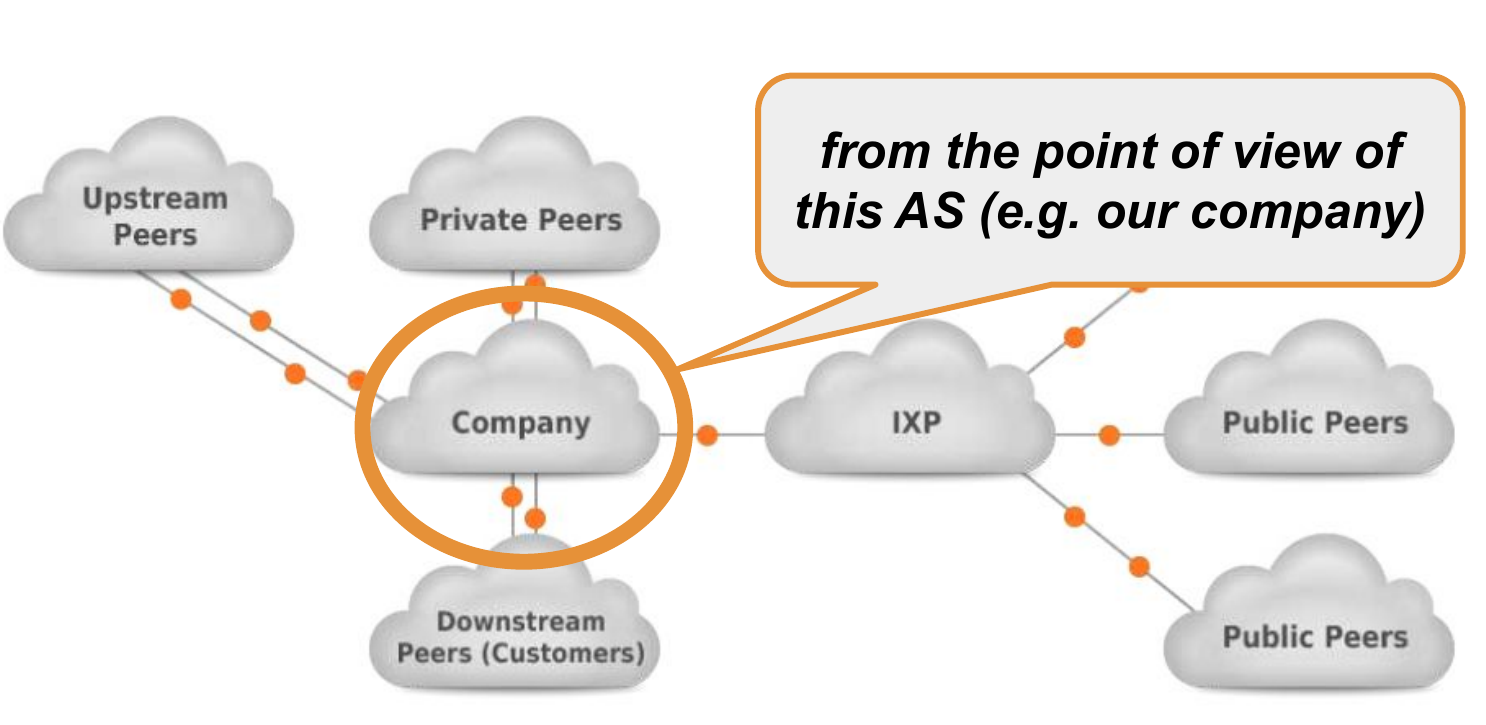
\includegraphics[scale=0.5]{../../immagini/bgp_rel}
\end{figure}\\\\
Occorre capire quali sono i diversi tipi di peers BGP:
\begin{itemize}
    \item transit provider
    \item customer AS: paga un altro AS per raggiungere il resto di Internet
    \item stub customer
    \item leaf customer: stub con un solo exit point
\end{itemize}
occorre considerare quali relazioni esistono fra i peers: la rete IXP è di layer 2 e viene usata dagli AS per connettere i loro router e connettersi agli altri AS.
\\È utile avere un IPX perché altrimenti occorrerebbe creare una connessione fisica fra i diversi peers BGP.
\\Un peer connesso ad un IXP viene chiamato \textbf{public peer}, tipicamente ogni ISP che partecipa ad una rete IXP ha il suo router di bordo, ci sarà poi una porta WAN del router connesso verso l'AS.
\\Negli IXP quindi ci colleghiamo ad altri AS e passiamo per la rete IXP solo per aggiungere gli altri AS.
\\Un \textbf{private peer} è connesso ad un link privato, quindi gli AS connessi hanno creato una connessione, nel caso del public peer non si usa come transito verso altri AS.
\\Lo stesso vale per i private peers, che gestiscono solo i prefissi dei customer.
\\Un \textbf{downstream peer}, anche detto customer peer prevede che l'ISP faccia advertising di tutta la routing table oppure delle rotte di default, i prefissi ricevuti dai customer sono rimandati a tutti i customer, i prefissi sono ricevuti perché l'AS è di transito per il customer, può essere necessario fare advertising di tutta la tabella nel caso di un customer multi-homed.
\\Abbiamo poi gli \textbf{upstream peers}, di solito è un ISP che usiamo per raggiungere l'Internet: a meno di non avere un 1st tier provider, occorre comprare la connettività per raggiungere il resto dell'Internet.
\\Annunciamo ad un upstream peer il nostro prefisso di casa e quelli degli altri customers.
\\Anche in questo caso o si riceve l'intera routing table oppure le route default, uno dei due in quanto dipende dalla topologia.
\\Le conseguenze di un root leaks sono
\begin{itemize}
    \item ridirezione del traffico tramite path non voluti
    \item quando un grande numero di rotte viene simultaneamente leakato, l'AS offending viene sovraccaricato e quindi si ha DoS o degrado delle performance
\end{itemize}

\subsection{Attacchi al data plane}
Due attacchi fondamentali:
\begin{itemize}
    \item DDoS, quindi il traffico è generato da diverse sorgenti distribuite.
    \\Per portarlo avanti, l'attaccante tipicamente usa pochi computer con buona potenza oppure un vasto numero di device di terza parte compromessi e non sospetti.
    \\In molti attacchi DDoS, l'IP sorgente dell'attaccante è spoofato così da non essere rintracciabile, o questo può appartentere ad un prefisso dirottato
    \item reflection aplification attack: spesso viene combinato con lo spoofing dell'IP sorgente.
    \\L'attaccante potrebbe usare un computer ad alta capacità con una larghezza di banda elevata o una botnet di dispositivi compromessi che mandano query a server di Internet gih performance.
        \\Per i servizi Internet che usano UDP (es DNS) le query e le risposte e le risposte sono contenute in un singolo pacchetto e lo scambio non richiede di stabilire una connessione fra sorgente e server.
\end{itemize}

\section{RPKI e BGP origin validation}
La prima cosa che facciamo è filtering: abbiamo gli Internet registries regionali ed i routing registries di Internet (sono DB dove c'è l'associazione fra AS e prefissi).
\\Gli oggetti presenti nell'IRR forniscono rotte dichiarate dagli operatori, è possibile col comando \texttt{whois} capire l'origine di un prefisso, facendo query ad un certo DB RIR.
\\L'informazione nel DB non erano autenticate, quindi è stato creato l'RPKI che è il PKI richiesto per certificare le informazioni di routing, vediamo la gerarchia
\begin{itemize}
\item IANA sono al top e allocano ai RIR (Europa, Asia etc...)
\item I RIRs sub-allocano risorse agli ISPs ed alle Enterprise
\item gli ISPs possono a loro volta sub-allocare ad altri ISPs
\item In alcune regioni i RIRs sub-allocano a dei LIRs, come ad esempio Telecom
\end{itemize}
RPKI è una autorità di certificazione locale offerta da tutti i RIR, la catena di certificati RPKI segue lo stesso ordine visto sopra, quindi IANA è il ground truth (avrà un certificato self-signed) che creerà un certificato per la RIR, la RIR firmerà a sua volta i certificati per gli ISP e così via.
\\Alla fine quindi, le RIR sono le trust anchor, in fondo alla catena abbiamo la ROA che è un binding fra prefisso, AS ed una lunghezza massima (per evitare di mandare rotte più corte), è un altro tipo di certificato ma come in ogni PKI abbiamo una catena di certificati.
\\Ci sono due modalità di certificazione delle risorse:
\begin{itemize}
    \item hosted: è il RIR che mantiene e gestisce le chiavi e fa le operazioni di RPKI 
    \item delegated: si delega la firma, il modello solamente più usato
\end{itemize}
Una volta che un ISP o una società (qualunque AS) riceve un certificato dalla RIR, è in grado di firmare le sue ROAs, può generare un EE-certificate ed usare la chiave privata per firmare.
\\Le funzionalità delle ROA, ovvero l'ultimo oggetto della catena, sono varie:
\begin{itemize}
	\item dichiara uno specifico AS come un origine autorizzata di annunci per il prefisso
	\item specifica uno o più prefissi ad un singolo numero di AS.
    \\Se viene specificata una lunghezza massima per un prefisso nella ROA, allora ogni altro prefisso più specifico con una lunghezza che non eccede la lunghezza massima può essere originato dall'AS specifico
    \item se il possessore ha un certificato della risorsa che lista più prefissi, può essere creata una ROA in cui alcuni o tutti i prefissi sono listati.
    \item le ROA possono essere create ed eventualmente firmate da un ISP per conto del cliente. 
\end{itemize}
Quindi, alla fine abbiamo questa situazione:\\
\begin{figure}[h!]
    \centering
    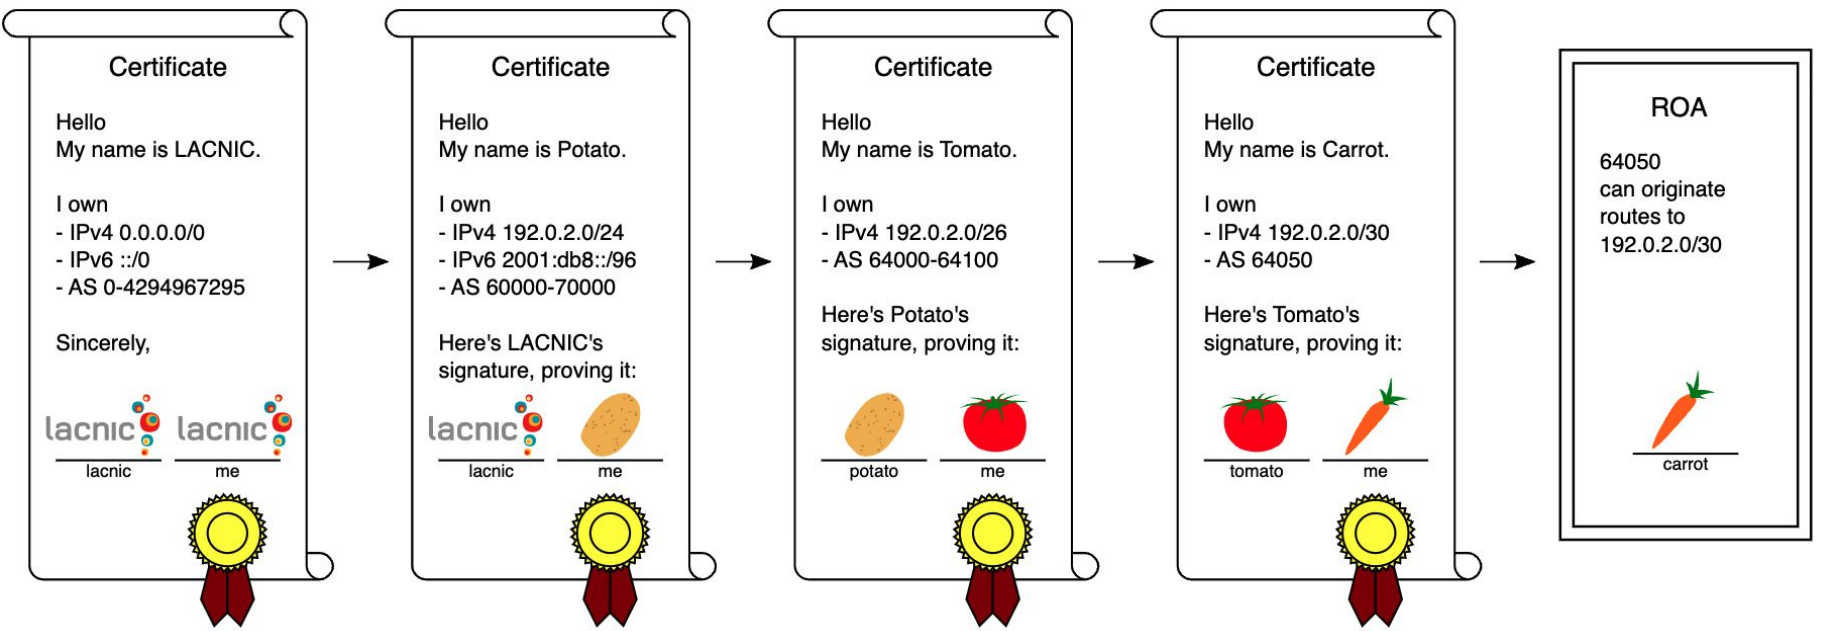
\includegraphics[scale=0.5]{../../immagini/rpki_chainpng}
\end{figure}\\\\
se si riceve un BGP update occorre verificare se questo è contenuto in un ROA valido, il che va fatto validando l'intera catena.
\\Come fanno i router ad ottenere questi certificati, perché le ROAs non sono trasportate dai messaggi di annuncio BGP: i router ottengono le ROAs ed una volta ricevuti gli annunci BGP fanno un controllo incrociato.
\\Le ROAs sono salvate nei RIRs o negli ISPs, un rotuer non vi accede direttamente, c'è una cache di ROAs negli ISPs, c'è un entità centrale dell'AS che prende le ROAs dalle repository dei server RPKI validatori (uno per ogni AS), che oltre a prendere le ROAs le verificano e le salvano nelle cache.
\\Infine, i router prendono col protocollo RTR le ROAs dalle cache.
\\Quando arriva un annuncio da un peer, il router controlla se il prefisso è in uno delle ROAs, non è il router che controlla la validità delle ROA in quanto il router le scarica già validate, si controlla anche se l'AS è quello giusto nella ROA.
\\Quindi, quando arriva un update, il router controlla solo in cache e quindi non è il router stesso a validare le ROA, bensì lo fa il server per motivi di scalabilità\\
\begin{figure}[h!]
    \centering
    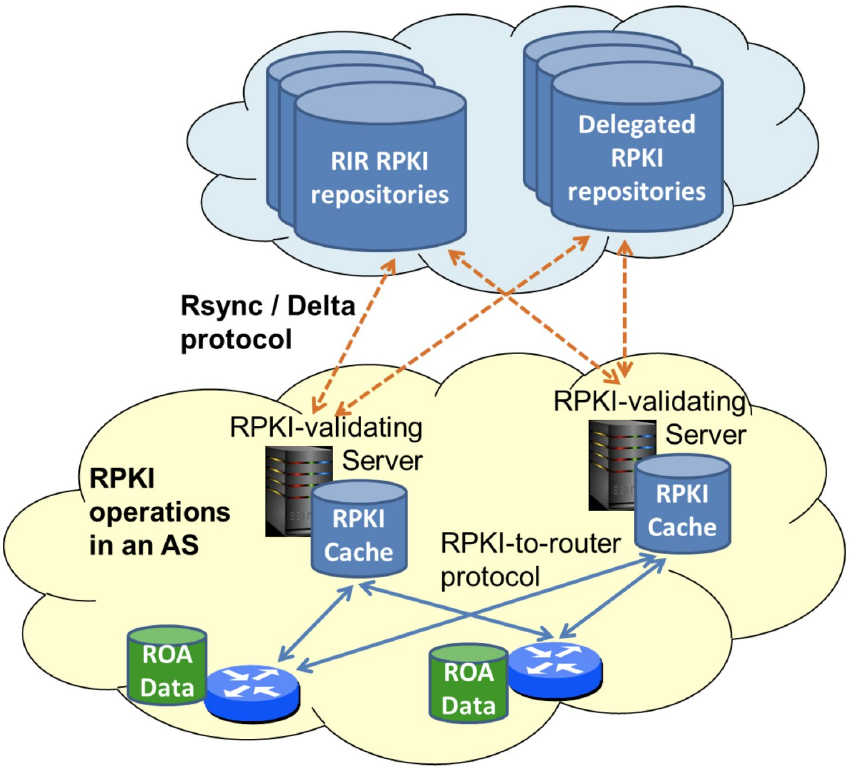
\includegraphics[scale=0.5]{../../immagini/rpki_valid}
\end{figure}\\\\
Un router BGP riceve quindi una lista di ROA validate, ed usa la lista con il BPG origin validation che è un tipo di processo di fast lookup.
\\Ovviamente c'è un problema sulla connessione fra router e server, ma si possono usare tutte le tecniche classiche, ad esempio TLS.
\\Il router quindi usa l'OV process per dire che una rotta mandata da un peer è valida se:
\begin{itemize}
	\item una rotta ha un'origine valida se la coppia (prefisso, AS origine )è valida e se \textbf{è valida la lunghezza massima}
	\item una rotta è invalida se c'è qualche tipo di mismatch
	\item una rotta è not found se non si può trovare nella lista delle ROAs
\end{itemize}
RPKI viene usato di solito solo per targare i prefissi, quindi si possono filtrare i BGP updates e dipende dall'AS l'azione che viene fatta.
\\Questo è come avviene la validazione dell'origine:\\
\begin{figure}[h!]
    \centering
    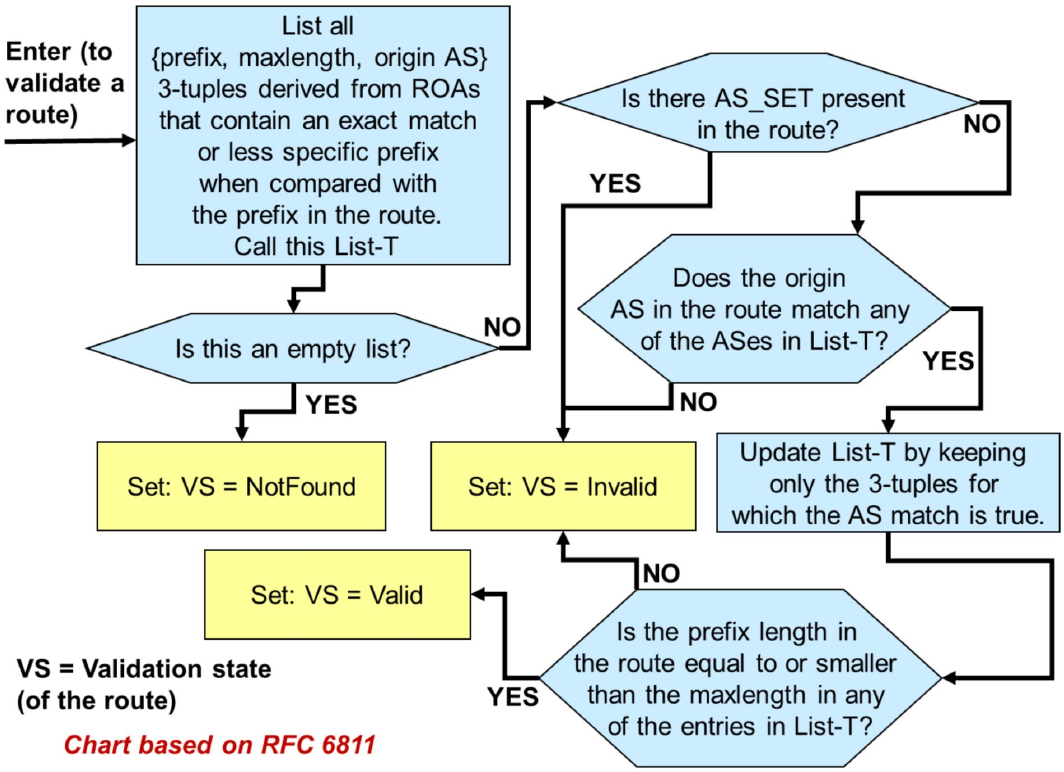
\includegraphics[scale=0.5]{../../immagini/orig_valid}
\end{figure}\\\\
C'è una web app molto simpatica di cloudflare che permette di validare un RPKI:
\begin{itemize}
	\item abbiamo il RIPE, che è la trust anchor, che è un prefisso gestito da Unidata
	\item abbiamo poi un certificato intermedio, che di nuovo è un "all" certificate (??) e firmato dal RIPE
	\item c'è poi il certificato di risorsa, che è una sub delegation
\end{itemize}
(slides per dettagli)
Ci sono una serie di implementazioni di RPKI.

\subsection{Forged-origin hijacks}
Anche con la PKI siamo ancora vulnerabili ad attacchi basati su forged-origin hijacking: è possibile forgiare un AS di origine per un qualunque update semplicemente aggiungendo un prefisso, come viene mostrato in seguito:\\
\begin{figure}[h!]
    \centering
    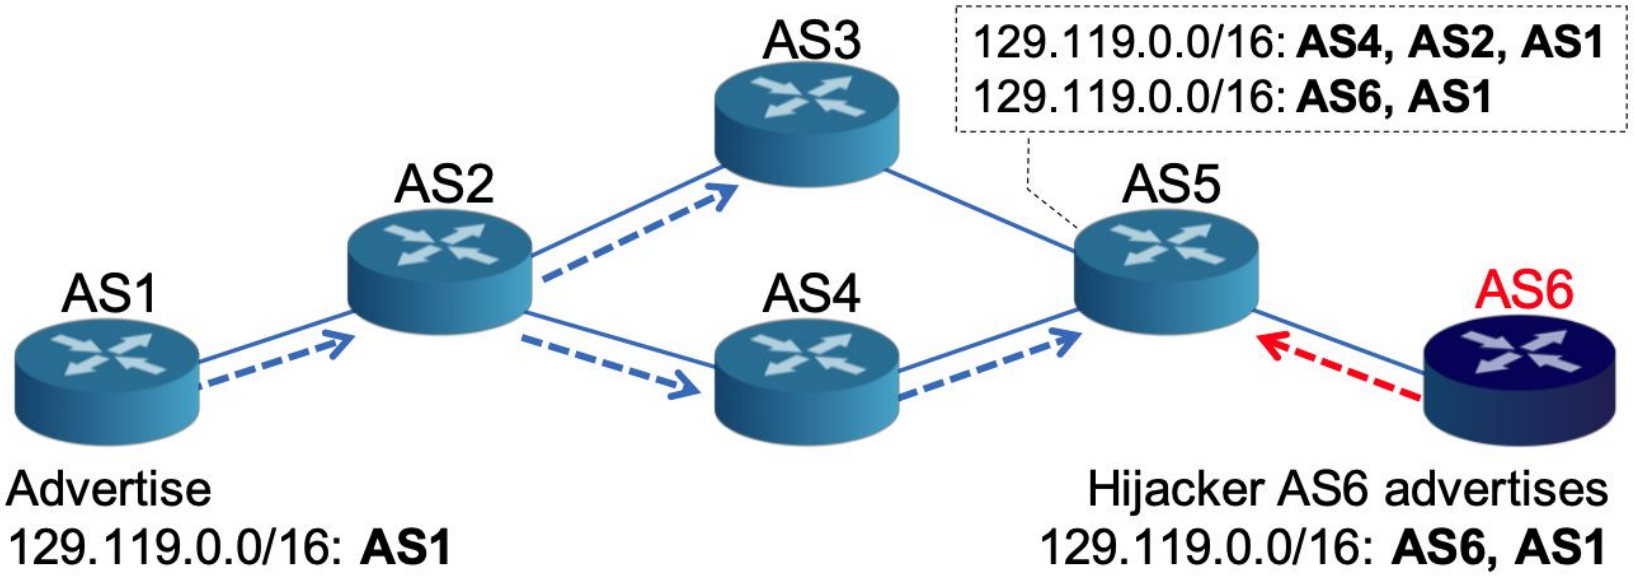
\includegraphics[scale=0.5]{../../immagini/orig_hijack}
\end{figure}\\\\
l'attaccante finge di essere nel mezzo fra la vera origine ed il router valido e non è nel path, ma comunque per il PKI risulta essere valido.
\\Le conseguenze sono le stesse dell hijacking, in quanto verrà preferita la rotta.
\\La soluzione è in BGPSec, protocollo pensato per proteggere questo tipo di attacchi:
\begin{itemize}
	\item ogni AS che implementa BGP-PV ha un router con un certificato
	\item ogni router nel path ha una chiave privata per firmare l'update BGP: l'owner della risorsa non genera solo la ROA
	\item le chiavi pubbliche dei router devono essere pubbliche
	\item l'update include la subject key 
	\item ogni AS riceverà molteplici firme da verificare
    \item se tutte le verifiche sono corrette e la validazione dell'origine torna, l'update BGP è corretto
\end{itemize}
La seguente figura esemplifica le cose:\\
\begin{figure}[h!]
    \centering
    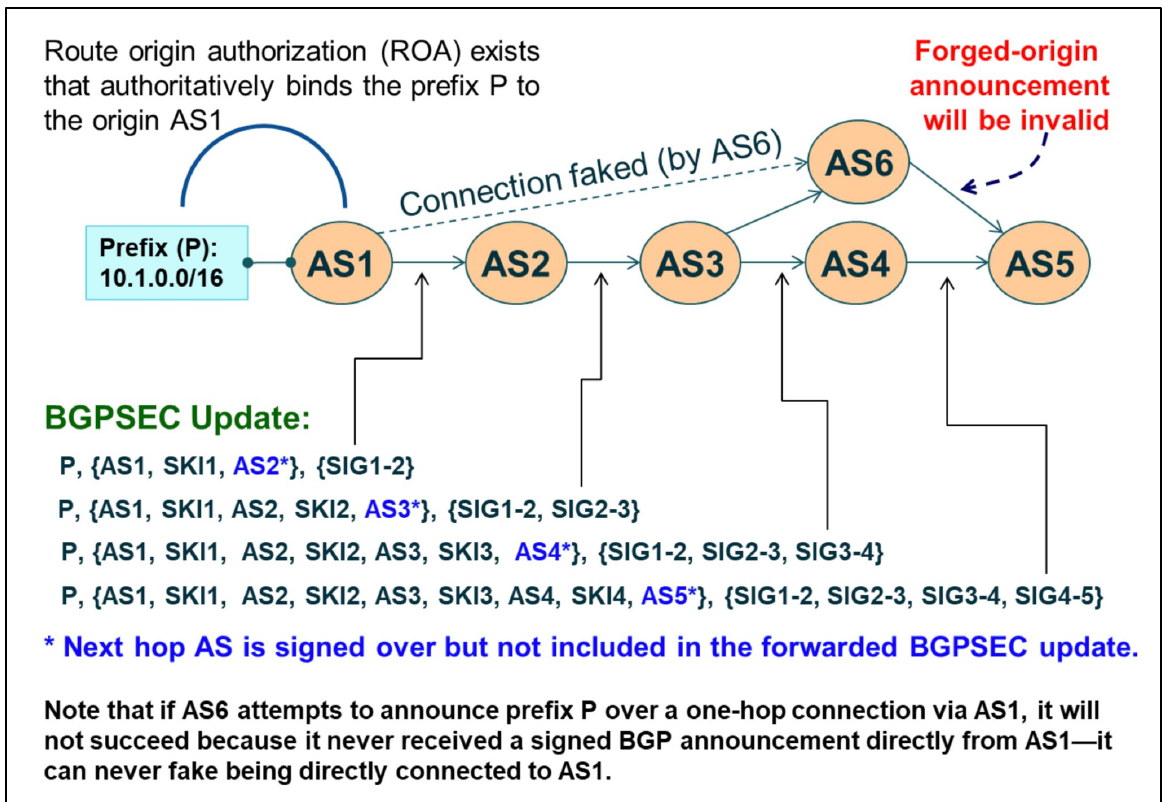
\includegraphics[scale=0.5]{../../immagini/bgp_path_valid}
\end{figure}\\\\
ogni router che riceve un update aggiunge alla firma il next-AS number, quindi in questo modo è impossibile forgiare una rotta.

\subsection{Prefix filtering}
RPKI fa binding crittografico, il filtering si basa su un insieme di policy per decidere se accettare un annuncio o no.
\\È il meccanismo più basico o meglio la prima soluzione per evitare di avere BGP leaking ed hijacking, non viene forzato ovunque ma è comunque una delle soluzioni.
\\Servono sia filtri inbound che outbound, in quanto possono esserci errori in cosa si manda in output ed ovviamente occorre filtrare cosa arriva da fuori.
\\Possiamo avere una visione come le ACL Cisco:\\
\begin{figure}[h!]
    \centering
    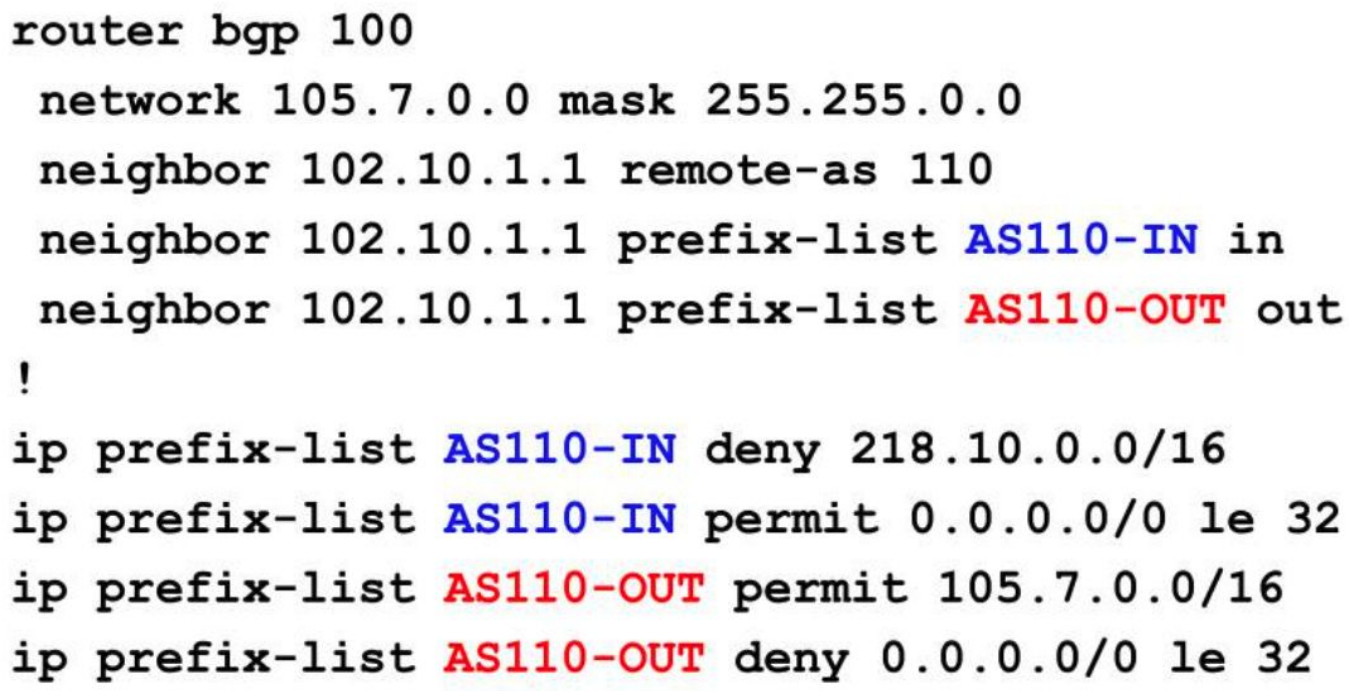
\includegraphics[scale=0.5]{../../immagini/acl_cisco}
\end{figure}\\\\
ogni cosa dipende dal tipo di relazione, quindi in base alla relazione che si ha col peer può essere necessario filtrare determinati prefissi ed altri no.
\\Possiamo avere diversi tipi di prefissi:
\begin{itemize}
	\item unallocated prefixes: prefissi non assegnati dallo IANA a nessuno.
    \\È buona pratica non accettare dei prefissi non allocati, è chiaramente un anomalia ricevere un prefisso di questo tipo
	\item special purpose prefix 
	\item prefissi controllati da un AS: se un AS riceve il suo stesso prefisso come advertisment è strano.
    \\Può esserci un loop, ma se lo ricevo da un AS path in cui non ci sono c'è qualcosa di strano
	\item prefissi che eccedono un limite dato: normalmente un ISP non accetta prefissi che siano troppo lunghi, ad esempio più di /24 per IPv4 o /48 per IPv6.
    \\È un attacco, perché una volta fatto hijacking si annuncia un prefisso più lungo di quello dell'owner reale.
    \\Alcuni operatori potrebbero decidere di rigettare prefissi anche troppo corti, ad esempio se un AS sa che il prefisso più lungo nella sua zona è /8 perché accettare uno /4?
	\item default route: la rotta può essere annunciata, ma solo in scenario specifici, ad esempio per customer single home, se il provider usa BGP deve annunciare la rotta di default, ma in generale va filtrata
	\item IXP LAN prefixes: un IXP dovrebbe annunciare il suo prefisso LAN o l'intero prefisso agli AS membri, ma si accetta solo dal root server dell'IXP e non da un altro peer BGP
\end{itemize}
Le raccomandazioni variano in base al tipo di relazione fra peers, ci sono diversi documenti pubblici che danno una lista di raccomandazioni dettagliate.
\\Un ISP può recuperare dagli RPKI routers tutte le rotte originariamente autorizzate corrispondenti agli AS che sa che sono fra i suoi customers.
\\Possiamo quindi usare RPKI per migliorare il filtering, filtrare è obbligatorio ed andrebbe fatto ovunque.

\subsection{Soluzioni al route leaks}
Se la rotta scoperta è nello stesso AS possiamo fare qualcosa, fra AS è più difficile
\begin{itemize}
    \item Nello stesso AS la soluzione prevede di taggare gli updates usando un attributo, che non si propaga nell'eBGP.
    \\Ogni update BGP viene taggato in ingresso per indicare che è stato ricevuto in eBGP da un customer, peer laterale o provider di transito.
    \\Al punto di egress, il router che invia applica una policy che usa il tagging:
        \begin{itemize}
            \item rotte ricevute da un cliente possono essere forwardate a qualunque peer;
            \item rotte ricevute da un peer laterale o da un provider di transito sono forwardate solo ai clienti
        \end{itemize}
    \item Per l'inter-AS è più complesso, ma c'è lavoro che continua per cercare una soluzione che non è maturo.
    \\Qui si cerca di rilevare e mitigare in caso di un leak di rotta che è già avvenuto.
    \\Difatti, se un leak si è propagato al di fuori di un AS, allora i peer AS o ogni altro AS lungo il percorso dovrebbe averlo ricevuto e bloccato.
    \\Una soluzione per questo problema è un work in progess nell IETF, difatti per la robustezza dell'Internet tecniche di detection e mitigazione dovranno essere implementate nelle capacità di prevenzione dell'intra AS.
\end{itemize}

\subsection*{Lab-013}
Configuriamo una topologia per usare BGP, vediamo cosa fare in base ai prefissi che riceviamo:
\begin{itemize}
	\item filtrare esplicitamente i prefissi assegnati, quindi manualmente. Non è scalabile
	\item filtrare esplicitamente gli AS\_PATH
	\item usares il community attribute: usiamo questa strada.
    \\Solo il provider edge router marca il pacchetto in arrivo e propaga l'udpate internamente con eBGP con il community value che utilizza.
    \\Quindi, gli altri nodi filtreranno non sul prefisso bensì sul community value
\end{itemize}


\subsection{Altri tipi di filtering}
Abbiamo visto solo strict filtering, quindi si accetta solo cosa si suppone di dover ricevere.
\\Possiamo fare filtering lasco, dove filtriamo:
\begin{itemize}
	\item local host
	\item indirizzi privati
	\item il nostro prefisso, che sappiamo per certo non può essere annunciato da altri
	\item loopback
	\item prefissi non allocati
	\item prefissi $>$ /24
\end{itemize}
va comunque usato quando non possiamo usare il filtering strict.
\\RPKI non è obbligatorio, quindi non possiamo solo buttare via i ROA non trovati, possiamo usare route-map, come mostrato in seguito:\\
\begin{figure}[h!]
    \centering
    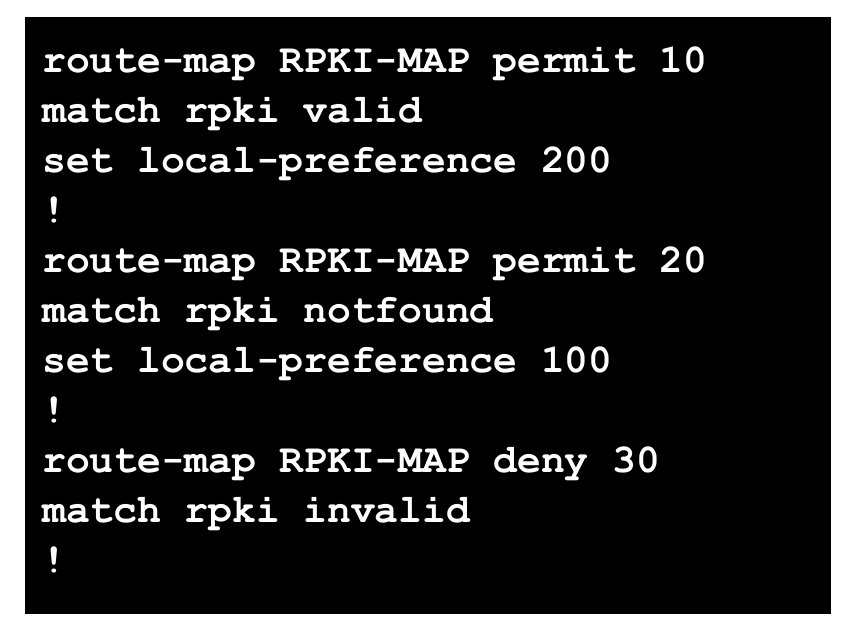
\includegraphics[scale=0.5]{../../immagini/route_map}
\end{figure}
con queste poche linee filtriamo in base alla ROA RPKI.
\end{document}
